Ziel dieses Versuchs ist es, die mechanischen Eigenschaften von Kupfer-Scherkörpern zu untersuchen und zu vergleichen:
\\
\vspace{0.05cm}
\begin{figure}[h]
    \centering
    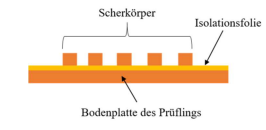
\includegraphics[scale=0.95]{Bilder/schematik.png}
    \caption{Versilberter Kupfer Scherkörper gesintert auf Kupferbodenplatte, (https://tinyurl.com/2p8ejcnv)}
    \vspace{0.2cm}
    \label{Abb.2: Versilberter Kupfer Scherkörper gesintert auf Kupferbodenplatte} 
\end{figure}\\

\begin{itemize}
\item Durchführung von Schertests an Prüflingen, wobei die Scherkörper durch Schubspannung mittels eines Schermeißels abgeschert werden.
\item Nach dem Scheren werden die einzelnen Prüfkörper auf Karteikarten aufgeklebt und mit dem zugehörigen, aus der Prüfsoftware abgelesenen Kraftwert beschriftet.
\item Die aufgenommenen Kraftwerte für alle Prüfkörper in einem Boxplot-Diagramm dargestellen.
\item Nach Abschluss der Scherversuche eine mikroskopische Untersuchung der Bruchstellen.
\item Im Fokus steht dabei die Identifikation und Analyse der verschiedenen Bruchmuster.
\item Das Ziel besteht darin, Unterschiede im Haftverhalten sowie in der Bruchcharakteristik der verwendeten Prüflinge zu erkennen und zu bewerten.
\item Gemessene Kraftwerte in Spannungen \textit{($\mathrm{N/mm^2}$)}  umrechnen.
\end{itemize}
